\noindent

\includegraphics[height=1.25cm]{images/pictograms/replication}

\includegraphics[height=1.25cm]{images/pictograms/benchmark}

\includegraphics[height=1.25cm]{images/pictograms/FEM}

\includegraphics[height=1.25cm]{images/pictograms/paraview}

%%%%%%%%%%%%%%%%%%%%%%%%%%%%%%%%%%%%%%%%%%%%%%%%%%%%%%%%%%%%%%%%%%%%%%%%%%%%%%%%%%%%%%%%%%%%%%%%%%%

\begin{flushright} {\tiny {\color{gray} python\_codes/fieldstone\_181/text.tex}} \end{flushright}

%\lstinputlisting[language=bash,basicstyle=\small]{python_codes/template_keywords.key}

\par\noindent\rule{\textwidth}{0.4pt}

\begin{center}
\inpython
{\small Code: \url{https://github.com/cedrict/fieldstone/tree/master/python_codes/fieldstone_181}}
\end{center}

\par\noindent\rule{\textwidth}{0.4pt}

Last revision: September 18th, 2025.

\par\noindent\rule{\textwidth}{0.4pt}

%%%%%%%%%%%%%%%%%%%%%%%%%%%%%%%%%%%%%%%%%%%%%%%%%%%%%%%%%%%%%%%%%%%%%%%%%%%%%%%%%%%%%%%%%%%%%%%%%%%

This \stone is a new take on \stone~40. 
The setup is identical. We here focus on the assembly of the FE matrix. 
Three methods are implemented and timed:
\begin{enumerate}
\item 
\item 
\item 
\end{enumerate}

\begin{center}
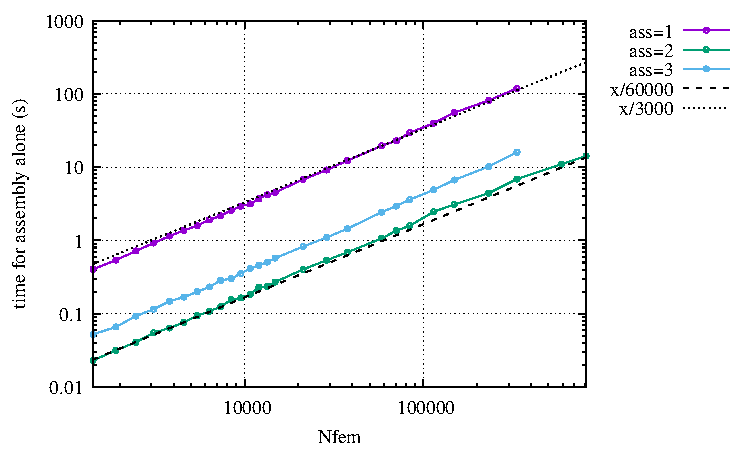
\includegraphics[width=8cm]{python_codes/fieldstone_181/RESULTS/times_assembly.pdf}
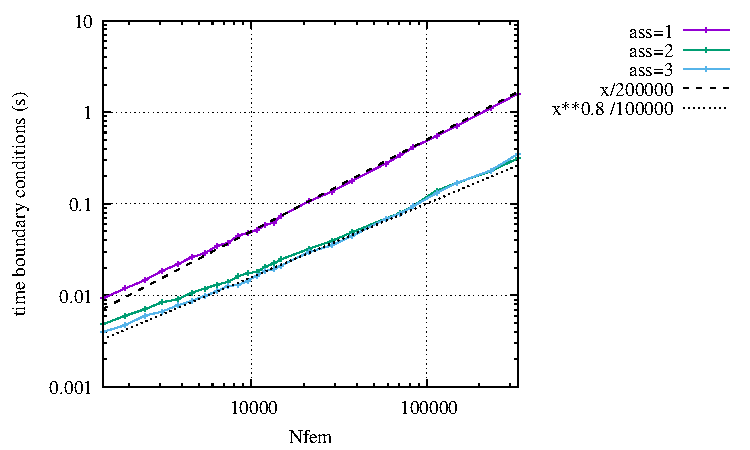
\includegraphics[width=8cm]{python_codes/fieldstone_181/RESULTS/times_bc.pdf}\\
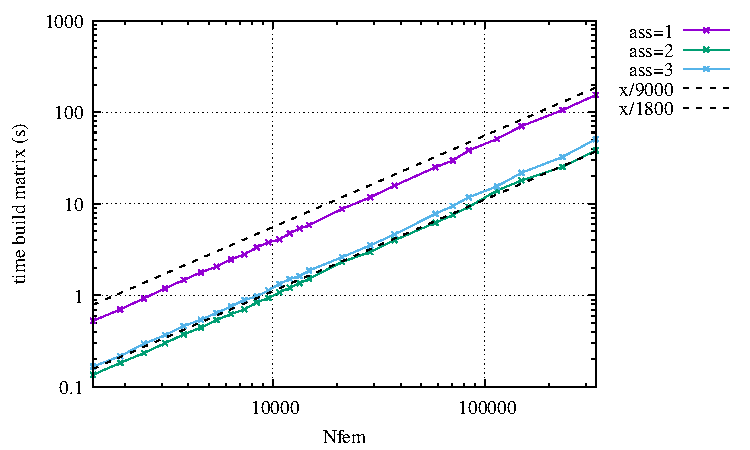
\includegraphics[width=8cm]{python_codes/fieldstone_181/RESULTS/times_build.pdf}
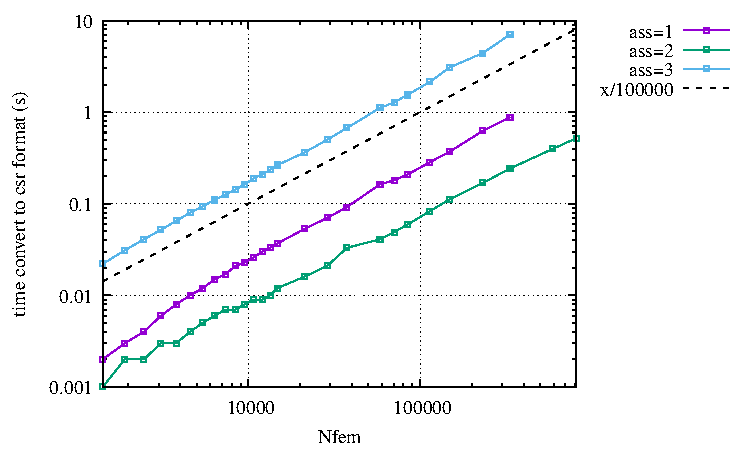
\includegraphics[width=8cm]{python_codes/fieldstone_181/RESULTS/times_convert.pdf}\\
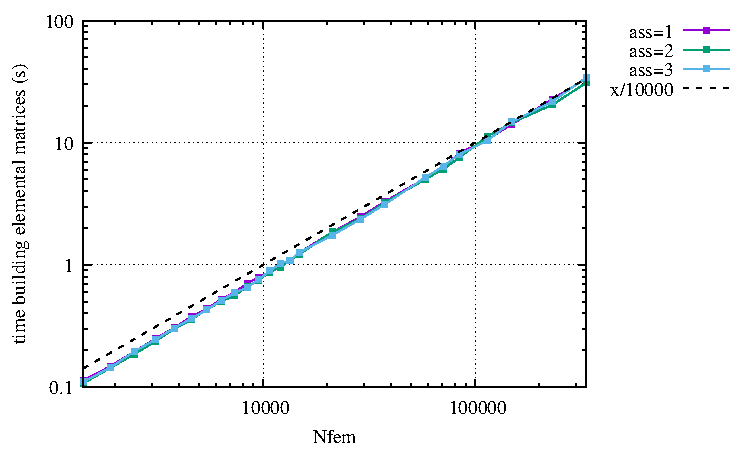
\includegraphics[width=8cm]{python_codes/fieldstone_181/RESULTS/times_matrices.pdf}
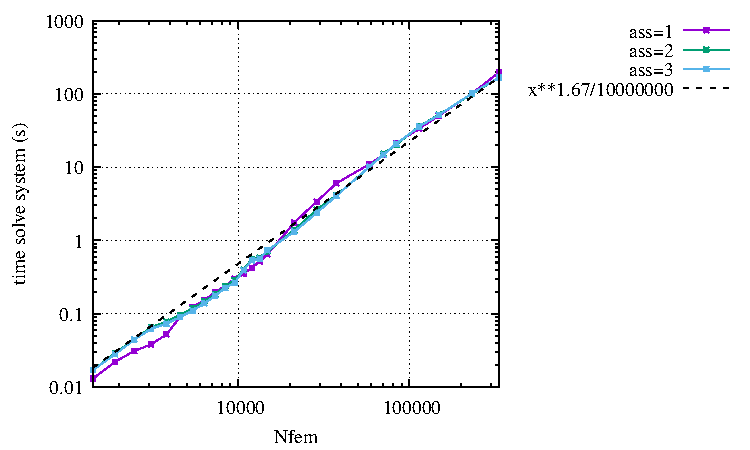
\includegraphics[width=8cm]{python_codes/fieldstone_181/RESULTS/times_solve.pdf}
\end{center}



\includegraphics[width=4cm]{./images/conclusion.png}


